\documentclass[11pt]{article}
%\documentclass[preprint, 10pt]{elsarticle}

% PACKAGES
\usepackage{graphicx, amsmath, amssymb, amsfonts, mathtools, mathrsfs, color}
\usepackage{comment, enumerate, tabularx}
\usepackage{natbib, hyperref, url}
\usepackage[margin=1in]{geometry}
%\usepackage[justification=RaggedRight]{caption}

%----------------------------------------------------------------------------%
%% LATEX DEFINITIONS
%----------------------------------------------------------------------------%
% Basic editing
\newcommand{\tocite}{{\color{blue}(to cite)}}
\newcommand{\vsp}[1]{\vspace{#1 pc} \noindent}
\newcommand{\np}{\newpage \noindent}
% Derivatives
\newcommand{\pd}[2]    { \frac{\partial #1} {\partial #2} }
\newcommand{\ppd}[2]  { \frac{\partial^2 #1}{{\partial #2}^2} }
\newcommand{\pdi}[2] { {\partial_#2} #1 }
\newcommand{\td}[2] { \frac{d #1} { d #2 } }
\newcommand{\grad}{\nabla}
\newcommand {\Lap} {\grad^2}
% Vectors and operators
\newcommand{\bvec}[1]{\ensuremath{\boldsymbol{#1}}}
\newcommand{\abs}[1]{\left| #1 \right|}
\newcommand{\norm}[1]{\left\| #1 \right\|}
\newcommand{\mean}[1]{\left< #1 \right>}
\newcommand{\eps}{\varepsilon}
\newcommand{\dx}{\, dx}
% Basic physical parameters and scales
\newcommand{\freqp}{f_p}
\newcommand{\etastd}{\eta_{\text std}}
% Parameters that change crossing the ADC
\newcommand{\depth}{d}
\newcommand{\dup}{\depth_{-}}
\newcommand{\ddn}{\depth_{+}}
\newcommand{\dupdn}{\depth_{\pm}}
\newcommand{\lam}{\lambda}
\newcommand{\lamup}{\lam_{-}}
\newcommand{\lamdn}{\lam_{+}}
\newcommand{\lamupdn}{\lam_{\pm}}
\newcommand{\lamfac}{N}
\newcommand{\drat}{\mathcal{D}}
\newcommand{\dratdn}{\drat_+}
\newcommand{\dratupdn}{\drat_{\pm}}
% Statistical quantities
\newcommand{\En}{\mathcal{E}}
\newcommand{\Mo}{\mathcal{M}}
\newcommand{\skw}{\text{skew}}
\newcommand{\skwdn}{\skw_+}
\newcommand{\var}{\text{var}}
\newcommand{\varup}{\var_-}
\newcommand{\vardn}{\var_+}
% Dimensionless parameters
\newcommand{\ampscale}{\mathcal{A}}
\newcommand{\lengthscale}{\mathcal{L}}
\newcommand{\timescale}{\mathcal{T}}
\newcommand{\epsup}{\eps_0}
\newcommand{\delup}{\delta_0}
% Hamiltonian stuff
\newcommand{\uhat}{\hat{u}}
\newcommand{\sympJ}{\mathcal{J}}
\newcommand{\vard}[2]{\frac{\delta #1}{\delta #2}}
\newcommand{\Ham}{\mathcal{H}}
\newcommand{\Hup}{\Ham^{-}}
\newcommand{\Hdn}{\Ham^{+}}
\newcommand{\Hupdn}{\Ham^{\pm}}
\newcommand{\Hthree}{\Ham_{3}}
\newcommand{\Htwo}{\Ham_{2}}
%\newcommand{\Fcnl}{\mathcal{F}}
% Truncated stuff
\newcommand{\Proj}{\mathcal{P}_{\Lambda}}
\newcommand{\uL}{u_{\Lambda}}
\newcommand{\HLupdn}{\Ham_{\Lambda}^{\pm}}
\newcommand{\SympL}{\sympJ_{\Lambda}}
% Gibbs and theta
\newcommand{\Gibbs}{\mathcal{G}}
\newcommand{\Gup}{\Gibbs^{-}}
\newcommand{\Gdn}{\Gibbs^{+}}
\newcommand{\Gupdn}{\Gibbs^{\pm}}
\newcommand{\thup}{\theta^{-}}
\newcommand{\thdn}{\theta^{+}}
\newcommand{\thupdn}{\theta^{\pm}}
\newcommand{\meanup}[1]{\mean{#1}_{-}}
\newcommand{\meandn}[1]{\mean{#1}_{+}}
\newcommand{\meanupdn}[1]{\mean{#1}_{\pm}}


% Experiments
\newcommand{\omavg}{\omega_0}
\newcommand{\omsig}{\sigma_{\omega}}
%----------------------------------------------------------------------------%

%----------------------------------------------%
%% TITLE
%----------------------------------------------%
\begin{document}

\title{The truncated KdV framework for modeling anomalous waves induced by abrupt depth changes}

% Title ideas
% Could include words "theory and experiments".
%Old idea: Deterministic and statistical truncated KdV models for anomalous waves induced by abrupt depth change
\author{
C.~Tyler Bolles\thanks{University of Michigan},
Andrew J.~Majda\thanks{Courant Institute of Mathematical Sciences}, 
M.~N.~J.~Moore\thanks{Florida State University}, 
Di Qi\thanks{Courant Institute of Mathematical Sciences} }
\maketitle

%----------------------------------------------------------%
% Intro
%----------------------------------------------------------%
\section{Introduction}

Rogue waves are abnormally large surface waves, defined by oceanographers as those that exceed twice the significant wave height. Though such waves were once dismissed as myth, they have now been recorded in oceans across the globe and pose a recognized threat to seagoing vessels and naval structures. Rogue waves, also variously known as freak or anomalous waves, have been observed both in deep and shallow water, and can be triggered by a variety of mechanisms, including anomalous wind-forcing, focusing due to variable bathymetry, and a deep-water modulational instability that goes by the name Benjamin-Feir. The common tie between these mechanisms is their ability to generate non-normal statistics in the surface displacement; when governed by Gaussian statistics, the likelihood of a rogue wave is extremely low, but these rare events occur much more frequently when surface statistics deviate from Gaussian. 

A recent series of laboratory \cite{bolles2019anomalous} and numerical investigations \cite{viotti2014} have demonstrated the emergence of anomalous wave statistics from abrupt variations in bottom topography. Since topographical variations are strictly one-dimensional, these studies can be viewed as offering a bare minimum set of conditions capable of generating anomalous wave statistics. In particular, the more complex mechanism of focusing by 2D bottom topography absent. The studies thus offer a paradigm system, with emergent anomalous statistical properties similar to that seen in more complex systems, but in a tractable context that is amenable to analysis.

Our particular focus is the laboratory experiments of Bolles et al.~\cite{bolles2019anomalous}, who demonstrated the emergence of anomalous statistics in a randomized wave-field upon encountering an abrupt depth change (ADC). In these experiments, an incoming wave-field is generated with nearly Gaussian statistics, and a plexiglass step placed near the middle of the tank creates the depth change. Upon passing into the region of shallower depth, the wave distribution skews strongly, with deviation from Gaussian being most pronounced a short distance downstream of the ADC. 
Inspired by these experimental observations, Majda et al.~\cite{majda2019statistical} laid out a theoretical foundation that accurately captures several aspects of the anomalous behavior. The theory is based on deterministic and statistical analysis of the truncated Korteweg–de Vries (TKdV) equations, and uses a combination of computational, statistical, and analytical tools. In follow-up work, Majda and Qi (cite) performed analysis on more severely truncated, lower-dimensional systems that were shown to exhibit many of the same anomalous features.

The purpose of the present manuscript is to expand on both the experimental findings of Bolles et al.~\cite{bolles2019anomalous} and the theoretical analysis of Majda et al.~\cite{majda2019statistical}, with particular emphasis on the synergy between the two; e.g.~experimental discoveries guiding theoretical developments and theoretical predictions inspiring new experimental tests. We present a range of previously unpublished experimental data, including statistics of the surface {\em slopes} (as opposed to only displacement data as published in \cite{bolles2019anomalous}, autocorrelation data, and some data on experiments in which the depth ratio was varied. We also expand on the theoretical treatment of \cite{majda2019statistical}, with emphasis on more direct link to experiments.

%~experimental discoveries guiding model developments, as well as new theoretical predictions inspiring new experimental tests.

%IDEA: Could comment on synergy, or close cooperation, between theory and experiments and the success thereof, then cite Ristroph erosion paper.


% combination
% draw close comparison
% with an even closer comparison between theoretical predictions and experimental measurements.



\vsp{4}

% ideal, paradigm, canonical, tractable

The purpose of this manuscript is to:
\begin{itemize}
\item Provide a more comprehensive treatment of the experiments and theory in combination. In particular, we make new comparisons between theory and experiments, which further confirm the predictive power of the theoretical framework.
\item Provide more thorough treatment of the link between physical system parameters and model parameters. This will elucidate the connection between theory and experiments. In particular, we flesh out details of non-dimensionalization, which were only briefly discussed in \cite{majda2019statistical} for the sake of brevity.
%more transparent connection to experimental parameters
\item Provide additional experimental measurements not presented in \cite{bolles2019anomalous}. For example, statistics on surface slope and autocorrelation.
\end{itemize}

%----------------------------------------------------------%
% Experiments
%----------------------------------------------------------%
\section{The experiments}

	As discussed in \cite{bolles2019anomalous}, the experiments consist of a long, narrow wave tank (6 m long x 20 cm wide x 30 cm high), with waves generated by plexiglass paddle at one end. The waves propagate through the tank and, roughly midway through, pass over an abrupt depth change (ADC), which is created by a plexiglass step. The waves continue to propagate through the shallower depth until reaching the far end of the tank, at which point their energy is dissipated by a horse-hair dampener. Since the dampener minimizes the backscatter, the waves in this experiment propagate primarily in one direction, from left to right in Fig.~\ref{fig1}. 

The pivoting motion of the paddle is driven by a 5-phase stepper motor. To generate a randomized incoming wave field, the paddle angle $\phi$ is specified by a precomputed psuedo-random signal
\begin{align}
\label{PaddleAngle}
& \phi(t) = \phi_0 + \Delta \phi \sum_{n=1}^N a_n \cos(\omega_n t+\delta_n) \, , \\
\label{anEq}
& a_n = \sqrt{\frac{2 \Delta \omega}{\pi^{1/2} \omsig}} \, 
\exp \left( -\frac{(\omega_n - \omavg)^2}{2 \omsig^2} \right) \, ,
\end{align}
(Literal copy and paste) Here, the angular frequencies are evenly spaced $\omega_n = n  \Delta \omega$ with step size $ \Delta \omega = (\omavg+4 \omsig)/N$, where $\omavg$ and $\omsig$ represent the mean and the bandwidth of $\omega$ respectively. We set $\omavg = \omsig = 12.5$ rad/s, corresponding to a peak forcing frequency of 2 Hz and bandwidth of 2 Hz. Importantly, the phases $\delta_n$ are uniformly distributed random variables. We fix $N = 3000$, which sets a fundamental period of $T = 300$ seconds.
	
 % Figure 1
%^^^^^^^^^^^^^^^^^^^^^^^^^^^^^^%
\begin{figure}%[!ht]
\begin{center}
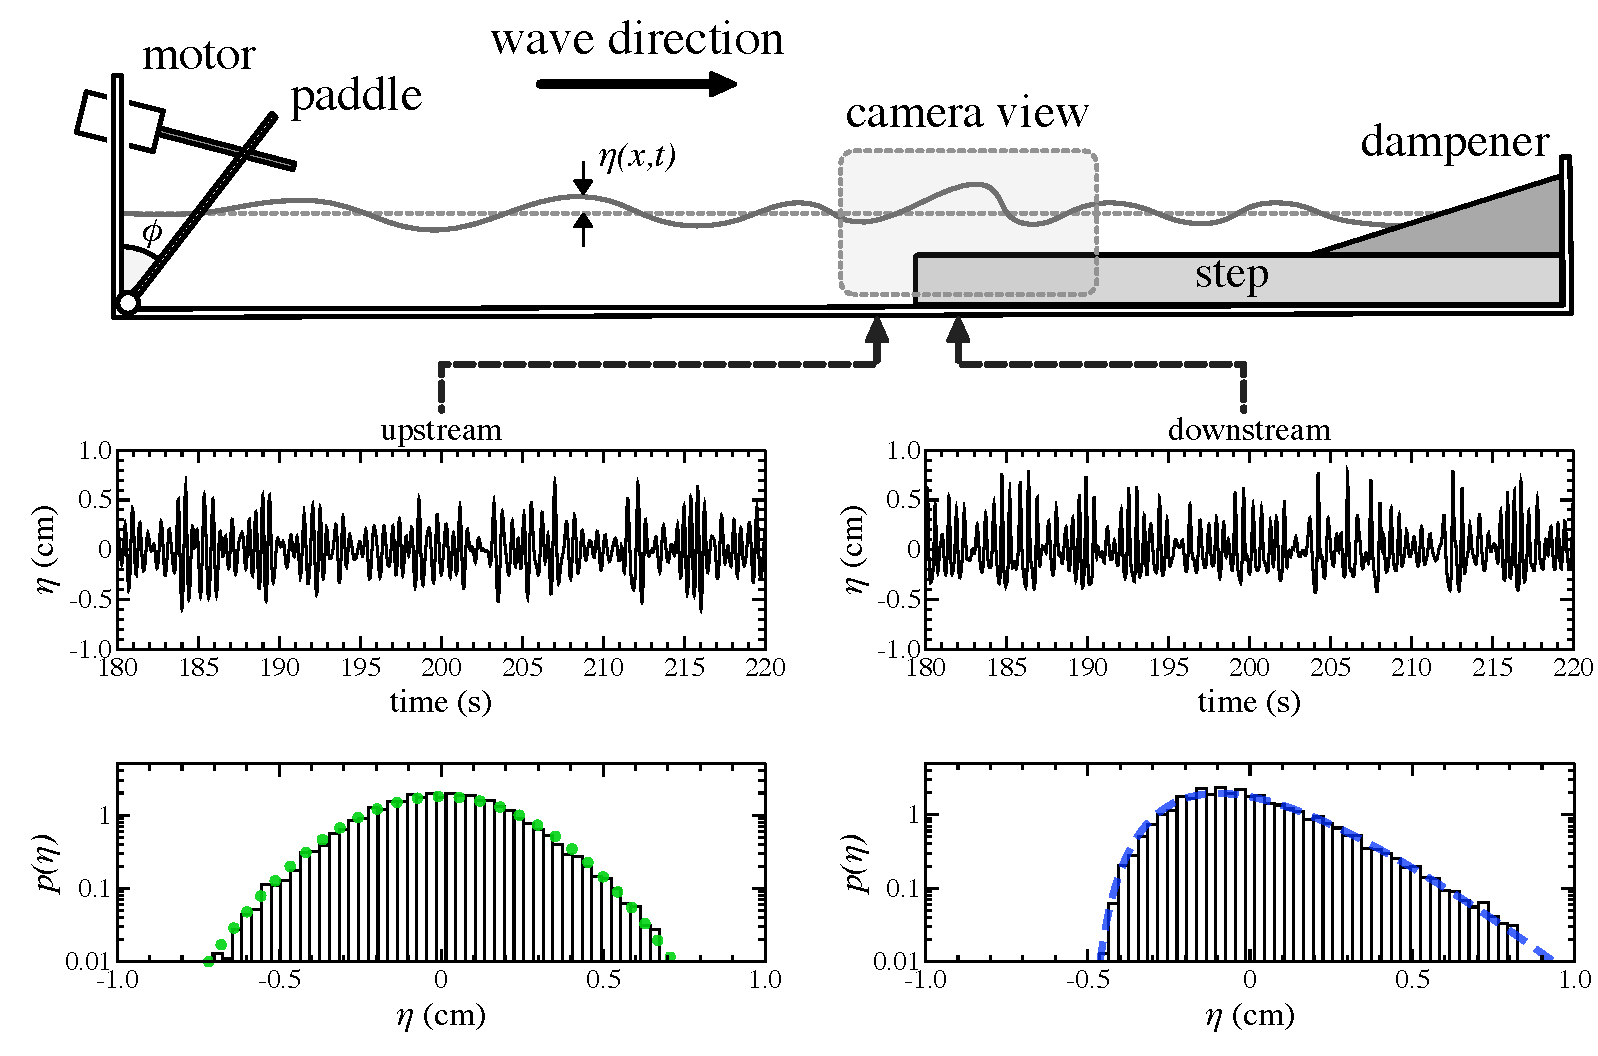
\includegraphics[width = 0.85 \linewidth]{Figs/fig1.pdf}
\caption{
(a) Experimental schematic. Reproduced from \cite{bolles2019anomalous}
}
%(b)--(c) Surface displacement measured at a representative upstream and downstream location. (d)--(e) Corresponding histograms.
\label{fig1}
\end{center}
\end{figure}
 %^^^^^^^^^^^^^^^^^^^^^^^^^^^^^^%

	The free surface is illuminated by light-emitting diodes running along the bottom of the tank and then imaged from the sideview with a Nikon D3300 at 60 frames per second. The illumination technique coupled with high pixel count of the camera allows surface displacements to be resolved with a accuracy better than 1/3 millimeter. Representative free surface measurements are shown in Figs.~\ref{fig2}(a)--(b) at a position upstream and downstream of the ADC. The corresponding histograms are shown in Figs.~\ref{fig2}(c)--(d).


 % Figure 2
%^^^^^^^^^^^^^^^^^^^^^^^^^^^^^^%
\begin{figure}%[!ht]
\begin{center}
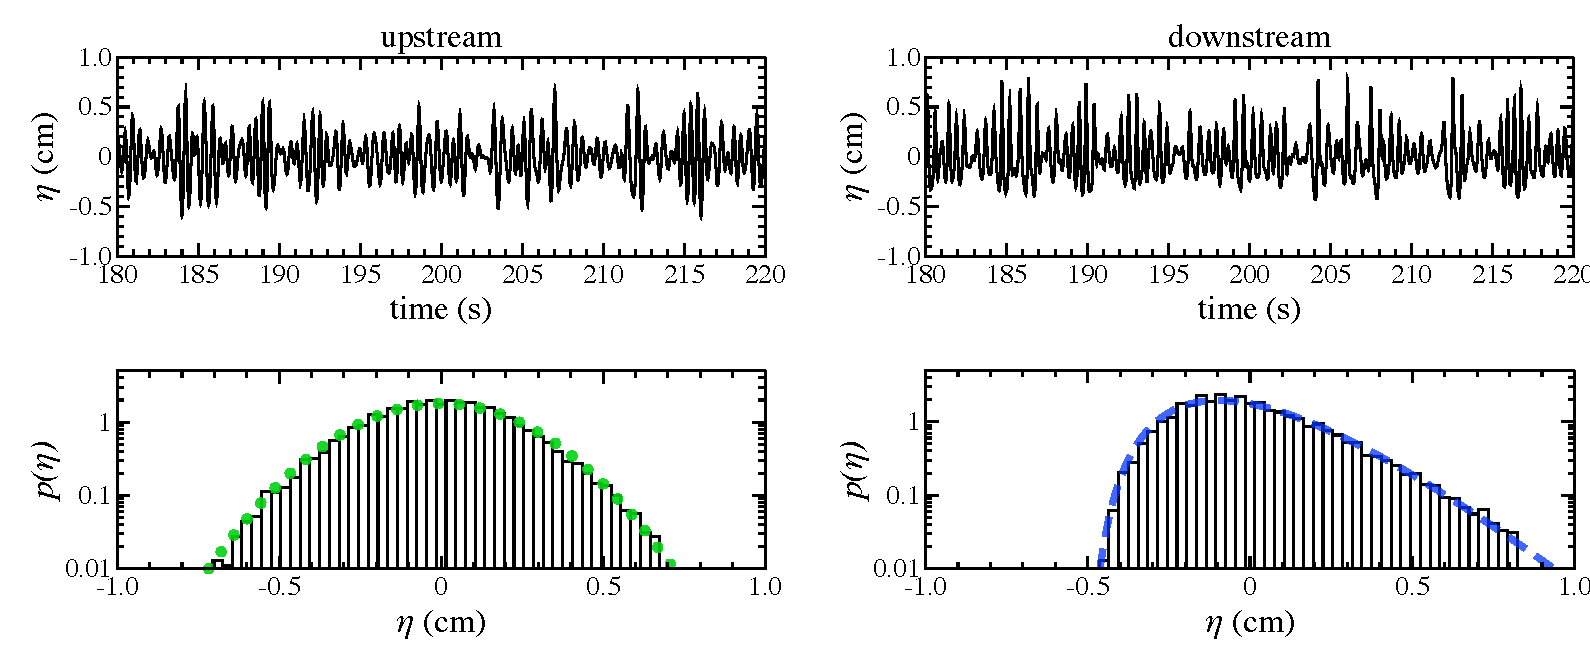
\includegraphics[width = 0.85 \linewidth]{Figs/fig2.pdf}
\caption{
(a)--(b) Surface displacement measured at a representative upstream and downstream location. (c)--(d) Corresponding histograms. Reproduced from \cite{bolles2019anomalous}
}
\label{fig2}
\end{center}
\end{figure}
 %^^^^^^^^^^^^^^^^^^^^^^^^^^^^^^%
 % Data from column 5 in MasterTimeSeries, Delta theta = 1.38 degrees, which is in between runs 5 and 6.
 
  % Figure 3
%^^^^^^^^^^^^^^^^^^^^^^^^^^^^^^%
\begin{figure}%[!ht]
\begin{center}
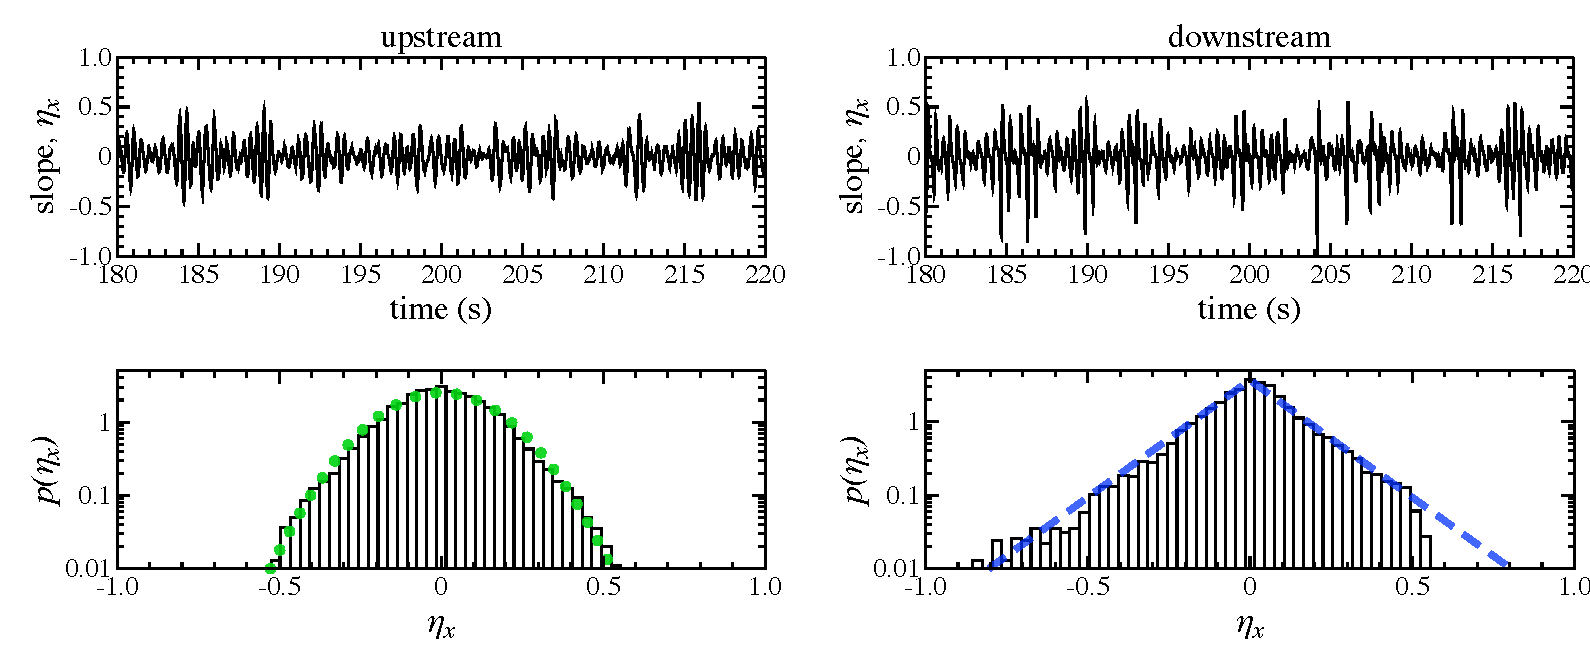
\includegraphics[width = 0.85 \linewidth]{Figs/fig3.pdf}
\caption{
(b)--(c) Surface slope measured at a representative upstream and downstream location. (d)--(e) Corresponding histograms. NEW PLOT.
}
\label{fig3}
\end{center}
\end{figure}
 %^^^^^^^^^^^^^^^^^^^^^^^^^^^^^^%
 
% Figure 4
%^^^^^^^^^^^^^^^^^^^^^^^^^^^^^^%
\begin{figure}%[!ht]
\begin{center}
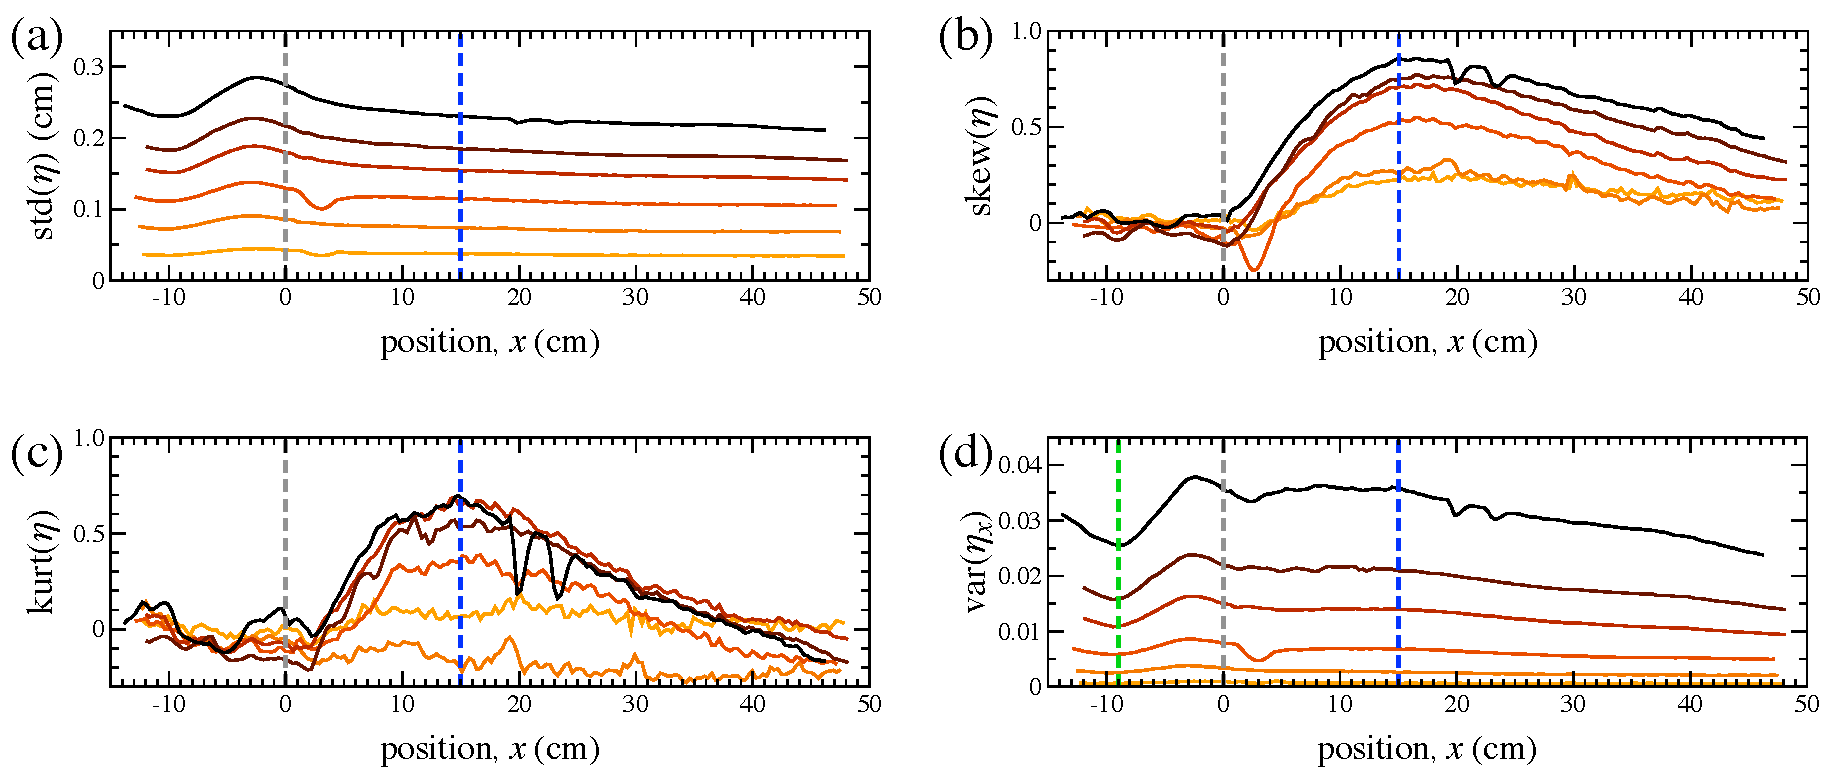
\includegraphics[width = 0.85 \linewidth]{Figs/fig4.pdf}
\caption{
Spatial statistics from the experiments.
}
\label{fig4}
\end{center}
\end{figure}
 %^^^^^^^^^^^^^^^^^^^^^^^^^^^^^^%
 
%----------------------------------------------------------%
% Theory
%----------------------------------------------------------%
\section{Theoretical framework}

%----------------------------------------------------------------------------%
% KdV
%----------------------------------------------------------------------------%
\subsection{The Korteweg–de Vries equation with variable depth}
Consider waves propagating unidirectionally in shallow water. Consider the surface displacement $\eta(x,t)$ and the reference frame moving with the local wave speed $\xi = x - ct$, where $c = \sqrt{g \depth}$ is the wave speed, $g$ gravity, and $\depth$ the local depth.
To first-correction in small amplitude, surface displacements are governed by the Korteweg–de Vries equation (KdV), which in dimensional form is given by \cite{whitham2011linear}
\begin{equation}
\label{KdV}
\eta_t + \frac{3 c}{2 \depth} \eta \eta_{\xi} + \frac{c \depth^2}{6} \eta_{\xi \xi \xi} = 0
\end{equation}
% This dimensional form is given by Whitham on p. 461, Eq. 13.98. I first got it from the Wolfram KdV, which gives the same equation.

We will primarily consider the case in which waves originate from a region of constant depth, encounter an abrupt depth change, and then continue in another region of constant depth. Thus, depth will be piecewise constant
\begin{align}
\depth = 
\begin{cases}
\dup \quad \mbox{if } x<0 \\
\ddn \quad \mbox{if } x>0
\end{cases}
\end{align}
Most often, we will consider waves moving into shallower depth, so that $\dup > \ddn$. 

The incoming waves are randomized and generated with a peak forcing frequency of $\freqp$, which gives rise to the following quantities
\begin{align}
&c = \sqrt{g \depth}
&&\mbox{\em local wave speed} \\
&\lam = c/\freqp = \sqrt{g \depth} / \freqp
&&\mbox{\em local peak wave length} \\
&\etastd = \mean{\eta^2}^{1/2} 
&&\mbox{\em standard deviation of displacement} \\
\end{align}
where $\mean{\cdot}$ indicates the mean of a quantity. 
Note that the characteristic wave speed $c = c_{\pm}$ and wavelength $\lam = \lamupdn$ each take different values upstream and downstream of the ADC. We remark that experimental measurements indicate that $\etastd = \mean{\eta^2}^{1/2}$ is nearly the same on both values of the ADC. Hence, we will not distinguish between upstream and downstream values of $\etastd$.
%
See Table \ref{paramtable} for a summary of important parameters.

% Table
%^^^^^^^^^^^^^^^^^^^^^^^^^^^^^^%
\begin{table}[h]%[htbp]
\begin{center}
\caption{Table of parameters}
\label{paramtable}
\begin{tabular}{l l l}
\hline \multicolumn{3} { c }{Parameters that are constant in a single experiment} \\
\hline Description & Notation and definition & Value in experiments \\
\hline
Peak forcing frequency		& $f_p$						& 2 Hz \\
Characteristic wave amplitude	& $\etastd = \mean{\eta^2}^{1/2} $		& 0.03--0.3 cm \\
Upstream depth			& $\dup$						& 12.5 cm \\
Downstream depth			& $\ddn$						& 3 cm (and varied) \\
Upstream wavelength		& $\lamup = \sqrt{g \dup}/f_p$		& 55 cm \\
Upstream wavelength		& $\lamdn = \sqrt{g \ddn}/f_p$		& 27 cm \\
%
Amplitude-to-depth ratio		& $\epsup = \etastd / \dup$			& 0.0024--0.024 \\
Depth-to-wavelength ratio		& $\delup = \dup / \lamup$		& 0.22 \\
Depth ratio				& $\dratdn = \ddn/\dup$			& 0.24 (and varied)
\end{tabular}
\end{center}
\end{table}
 %^^^^^^^^^^^^^^^^^^^^^^^^^^^^^^%
 
 
%----------------------------------------------------------------------------%
% Nondimensionalization
%----------------------------------------------------------------------------%
\subsection{Nondimensionalization and relation to experimental scales}

In this section, the variable-depth KdV equation \eqref{KdV} will be recast into a dimensionless form chosen for convenience in working with the statistical-mechanics framework introduced in \cite{majda2019statistical}. Since the choice of normalization not unique, it is instructive to first introduce a generic normalization to facilitate comparison with other choices. To this end, consider characteristic scales, $\ampscale, \lengthscale, \timescale$ for the wave amplitude, longitudinal length, and time respectively, which can remain unspecified for the moment. We introduce the dimensionless variables
\begin{align}
&u = \eta / \ampscale
&&\mbox{\em dimensionless surface displacement} \\
&\tilde{x} = \xi / \lengthscale
&&\mbox{\em dimensionless position (in moving frame)} \\
&\tilde{t} = t / \timescale
&&\mbox{\em dimensionless time}
\end{align}
Recasting \eqref{KdV} in terms of these variables gives the generic dimensionless KdV equation:
\begin{equation}
u_t + \frac{3}{2} \left( \frac{c \timescale \ampscale}{\lengthscale \depth} \right) u u_x 
+ \frac{1}{6} \left( \frac{c \timescale \depth^2}{\lengthscale^3} \right) u_{xxx} = 0
\end{equation}
We have dropped the tilde notation above for simplicity and will henceforth use tildes only in cases of possible ambiguity.

Now it is possible to choose the scales $\ampscale, \lengthscale, \timescale$ for ease in working with a particular framework. We choose the following scales,
\begin{align}
\label{scales}
\ampscale = \pi^{1/2} \, \etastd \, , \qquad
\lengthscale = \frac{\lamfac \lam}{2 \pi} \, , \qquad
\timescale = \frac{\lamfac \lam}{2 \pi \freqp \depth}
\end{align}
where $\lamfac$ is an integer to be chosen later. 
The explanation for these choices is as follows. First, we have chosen the characteristic amplitude, $\ampscale$, above to normalize the energy of the state-variable $u$ to unity, as will be demonstrated in Section \ref{tKdVSec}. Second, regarding $\lengthscale$, recall that $\lam$ is the characteristic wavelength corresponding to the peak forcing frequency $\freqp$ in the experiments. If only integer multiples of $\freqp$ were imposed (e.g.~lower frequencies were not present), then the forcing would produce waves that are periodic over lengthscale $\lam$. Since lower frequencies do exist, strict periodicity is not satisfied, but rather waves may be nearly periodic over the physical domain $\xi \in [-\lam/2, \lam/2]$. The approximation of near-periodicity becomes more accurate if integer multiples of $\lam$ are considered, i.e.~$\xi \in [-\lamfac \lam/2, \lamfac \lam/2]$. Thus, we have chosen $\lengthscale$ above so that the dimensionless domain of consideration is $\tilde{x} \in [-\pi, \pi]$ and periodic boundary conditions on $u$ can be  imposed on over this domain with accuracy that increases with $\lamfac$. Lastly, regarding $\timescale$, the most basic timescale in the experiments is simply $\freqp^{-1}$, i.e.~the period of waves passing a fixed reference point. Of course, the leading-order behavior in shallow water is simple translation of waves with uniform speed $c$. The KdV equation provides the first correction to this behavior and describes dynamics that evolve over longer timescales. Hence we have rescaled $\freqp^{-1}$ by the factor $N \lam/(2 \pi \depth) \gg 1$, which provides a suitably long timescale and is in line with previous normalizations \cite{johnson1997modern}. The scales $\lengthscale$ and $\timescale$ change value across the ADC, which is important to note when comparing the theory against experimental measurements.

With the above choices, the dimensionless KdV takes the form
\begin{align}
\label{dimlessKdV}
&u_t + C_3 \drat^{-3/2} \, u u_x + C_2 \drat^{1/2} \, u_{xxx} = 0
\qquad \text{for } x \in [-\pi,\pi] \\
&C_3 = \frac{3}{2} \pi^{1/2} \epsup \delup^{-1} \, , \quad
C_2 = \frac{2 \pi^2 \delup}{3 \lamfac^2} 
%C_2 = \frac{\pi^2 \delup}{6 \lamfac^2} 
\end{align}
The constants $C_3$ and $C_2$ do {\em not} change value crossing the ADC and are given in terms of the dimensionless parameters
\begin{align}
&\epsup = \etastd / \dup
&&\mbox{\em upstream amplitude-to-depth ratio} \\
&\delup = \dup / \lamup
&&\mbox{\em upstream depth-to-wavelength ratio}
\end{align}
The reason for the subscripts $3$ and $2$ will become evident in the next section. 

Meanwhile, the dimensionless depth $\drat = {\depth}/{\dup}$ {\em does} change value across the ADC since the depth $\depth$ changes. Recall that the reference frame of \eqref{dimlessKdV} moves with the local wave speed via the variable $\xi = x-ct$ from \eqref{KdV}. Thus, the ADC is met at some time $T_{ADC}$, and for simplicity we set $T_{ADC} = 0$. Therefore, we can regard $\drat$ is a piece-wise constant function of dimensionless time
\begin{equation}
\label{dratpw}
\drat = 
\begin{cases}
1 		&\quad \mbox{for } {t}<0 \\
\dratdn = {\ddn}/{\dup} 	&\quad \mbox{for } {t}>0
\end{cases}
\end{equation}

A few comments are in order. First, we note that the original formulation of this theory utilized a slightly different normalization \cite{majda2019statistical}, with identical powers of $\drat$ in \eqref{dimlessKdV} but with different expressions for the other dimensionless parameters. These differences are purely cosmetic, and we have made the choices above simply to facilitate comparison against the experiments. Second, an alternate formulation of the variable-depth KdV equation exists in which it is conjectured that the product $\depth^{1/4} \eta$, rather than $\eta$, varies continuously across the ADC \cite{johnson1997modern}. Of course, that assumption implies a discontinuity in surface displacement, which, though small, is physically unrealistic. We have chosen to enforce continuity of surface displacement in the above on the basis of physical realism. Using the alternative formulation would simply modify the power of $\drat$ in the second term of \eqref{dimlessKdV} by 1/4, i.e.~$\drat^{-7/4}$ instead of $\drat^{-3/2}$. Hence, all of the results discussed below would still hold qualitatively in this alternate formulation, with only slight quantitative modifications.

%NOTE: Perhaps we should be more specific about comparing to the dimensionless parameters in our PNAS paper \cite{majda2019statistical}, BUT the expressions for E0 and L0 given in the PNAS paper do not match with what I calculate comparing to the above. Plus, it seems like it could only add confusion.
 

%----------------------------------------------------------------------------%
% Hamiltonian
%----------------------------------------------------------------------------%
\subsection{Hamiltonian structure of KdV}
\label{HamiltonianSection}

The variable-depth KdV \eqref{dimlessKdV}, though not Hamiltonian throughout the entire domain, admits a Hamiltonian structure on each side of the ADC. Indeed, \eqref{dimlessKdV} can be expressed as
\begin{align}
\partial_t{u} = \sympJ \vard{\Hupdn}{u}
\end{align}
where $\sympJ = \pdi{}{x}$ is the symplectic operator and $\Ham = \Hupdn$ is the Hamiltonian, which will take different forms on either side of the ADC. It is convenient to decompose the Hamiltonian into a so-called cubic and quadratic component, given respectively by
\begin{align}
\label{H3H2}
\Hthree = \frac{1}{6} \int_{-\pi}^{\pi} u^3 \dx	\, , \qquad
\Htwo = \frac{1}{2} \int_{-\pi}^{\pi} u_x^2 \dx	\, .
\end{align}
Then the Hamiltonian can be expressed as
\begin{equation}
\label{Hamiltonian}
\Hupdn = C_2 \dratupdn^{1/2} \, \Htwo - C_3 \dratupdn^{-3/2} \, \Hthree
\end{equation}
where $\drat = \dratupdn$ changes value across the ADC. More explicitly, substituting \eqref{dratpw}, the separate upstream and downstream Hamiltonians are
\begin{align}
&\Hup = C_2 \, \Htwo - C_3 \, \Hthree 						&& \text{for } t<0 \\
&\Hdn = C_2 \dratdn^{1/2} \, \Htwo - C_3 \dratdn^{-3/2} \, \Hthree	&& \text{for } t>0
\end{align}
The above formulation differs cosmetically from some previous ones \cite{abramov2003hamiltonian, bajars2013weakly, majda2019statistical}, which used the opposite sign in both $\sympJ$ and $\Ham$. With that sign convention, Majda et al. 2019 found that a {\em negative} inverse temperature is required to accurately describe the experimental observations \cite{majda2019statistical}. We have chosen the sign convention above (which also happens to be consistent with Lax \cite{lax1975periodic}) so that a {\em positive} inverse temperature could be used and thus fit the theory into the most conventional form of statistical mechanics.

% Notes for myself on the sign change: Abramov CPAM 2003, Bajars Nonlinearity 2013, and our 2019 PNAS paper all use J = -d/dx with the opposite sign in the Hamiltonian. However, I was able to easily find several references online that use J = d/dx, so there is nothing wrong with it. The exact criteria that J has to satisfy are listed in the CPAM 2003 paper, and J = d/dx satisfies all these criteria just as well as J = -d/dx does.

We introduce two important invariants of KdV, the momentum and the energy
\begin{align}
\label{MomEn}
\Mo[u] \equiv \int_{-\pi}^{\pi} u \dx \, = 0 , \qquad
\En[u] \equiv \frac{1}{2} \int_{-\pi}^{\pi} u^2 \dx = 1
\end{align}
As indicated above, the momentum of $u$ vanishes since it is measured as displacement from equilibrium. Second, by the scale chosen for $\ampscale$ in \eqref{scales}, the energy has been normalized to unity.

The evolution of any functional $\mathcal{F}[u]$ is given by 
\begin{align}
\partial_t \mathcal{F} = \{ \mathcal{F}, \Ham \} = \int_{-\pi}^{\pi} \vard{\mathcal{F}}{u} \sympJ \vard{\Ham}{u} \dx
\end{align}
where again $\Ham = \Hup$ if $t<0$, and $\Ham = \Hdn$ if $t>0$ and $\{\}$ is the Poisson bracket induced by $\sympJ$.



%----------------------------------------------------------------------------%
% Truncated KdV
%----------------------------------------------------------------------------%
\subsection{Truncated KdV}
\label{tKdVSec}

We now introduce the truncated KdV (TKdV) system, which is the main focus of this study. Consider the Fourier series of the state variable
\begin{align}
&u(x,t) = \sum_{k=-\infty}^{\infty} \uhat_k e^{i k x} \, , \\
\label{uhat}
&\uhat_k = \frac{1}{2 \pi} \int_{-\pi}^{\pi} u(x) e^{-i k x} \dx
\end{align}
Since $u$ is real valued, we have $\uhat_{-k} = \uhat_{k}^*$ and since momentum vanishes $\uhat_0 = 0$.
Next, consider the Galerkin truncation at wave number $\Lambda$
\begin{align}
\uL(x,t) = \Proj u =
\sum_{\abs{k} \le \Lambda} \uhat_k e^{i k x} \, , \qquad
\end{align}
where $\Proj$ is a projection operator and \eqref{uhat} still holds. Projecting the KdV equation \eqref{dimlessKdV} onto the finite dimensional space gives the truncated KdV equation (TKdV)
\begin{align}
\label{TKdV}
&\pd{\uL}{t} +  \frac{1}{2} C_3 \drat^{-3/2} \,\Proj (\uL)^2 + C_2 \drat^{1/2} \, \frac{\partial^3 \uL}{\partial x^3} = 0
\qquad \text{for } x \in [-\pi,\pi] \\
&C_3 = \frac{3}{2} \pi^{1/2} \epsup \delup^{-1} \, , \quad
C_2 = \frac{2 \pi^2 \delup}{3 \lamfac^2}
\end{align}
Note the additional projection operator in front of the quadratic term $\uL^2$, which removes the aliased modes of wavenumber larger than $\Lambda$. The constants $C_3$ and $C_2$ are the same as before and have been repeated here for convenience. 

Remarkably, the TKdV system \eqref{TKdV} retains nearly the same Hamiltonian structure described in Section \ref{HamiltonianSection}, with the only modification being the inclusion of the projection operator \cite{bajars2013weakly, majda2019statistical}. The piecewise defined Hamiltonian for TKdV is given by
\begin{equation}
\label{TruncHamiltonian}
\HLupdn = C_2 \dratupdn^{1/2} \, \Htwo[\uL] - C_3 \dratupdn^{-3/2} \, \Hthree[\uL]
\end{equation}
where $\Hthree$ and $\Htwo$ the defined exactly as before \eqref{H3H2}, but now are simply applied to the projected variable $\uL = \Proj u$.
Then TKdV \eqref{TKdV} can be expressed as
\begin{align}
\partial_t {\uL} = \partial_x \Proj \, \vard{\HLupdn}{\uL}
\end{align}
where the truncated symplectic operator is $\SympL = \partial_x \Proj$.
% Note: Bajars 2013 has some important details on the Hamiltonian on the truncated system.

The momentum and energy defined in \eqref{MomEn} remain invariants of TKdV, with the same normalization values $\Mo[\uL] = 0$ and $\En[\uL] = 1$. Note that Parseval's identity gives
\begin{equation}
\En[\uL] = 2 \pi \sum_{k=1}^{\Lambda} \abs{\uhat_k}^2 = 1
\end{equation}
% The above agrees with the first line on top of p. 4 in Majda and Qi J Stat Phys 2019.
As has been noted before, the (untruncated) KdV system possesses an infinite sequence of additional invariants \cite{lax1975periodic, whitham2011linear}. The projected counterparts of these invariants, however, are not necessarily invariants of the truncated system.

% Is it true that the only 3 known invariants of TKdV are the ones mentioned here: momentum, energy, and Hamiltonian.


%----------------------------------------------------------------------------%
% Gibbs
%----------------------------------------------------------------------------%
\subsection{Mixed microcanonical-canonical Gibbs ensemble}

In examining statistical mechanics of this Hamiltonian system, we will appeal to the idea of a {\em mixed microcanonical-canonical} Gibbs ensemble, as originally introduced in \cite{abramov2003hamiltonian} for the Burgers-Hopf system. Specifically, this ensemble is microcanonical in the energy, with a fixed energy value, and it is canonical in the Hamiltonian. By fixing the energy and hence confining to a compact set, this construction avoids the divergence at infinity that would occur for a simple canonical ensemble and hence yields a normalizable distribution. This framework applies equally well to the truncated or untruncated system and hence we will not distinguish between the two.

The Hamiltonian on either side of the ADC, $\Ham^{\pm}$, generates a corresponding mixed ensemble, or Gibbs measure given by 
\begin{align}
\Gupdn = C_{\thupdn} \exp(-\thupdn \Hupdn) \delta(\En - 1)
\end{align}
Here $\theta = \thupdn$ is the inverse temperature and $C_{\theta}$ a constant (inverse of the partition function) that depends on $\theta$. Each measure has corresponding ensemble mean $\mean{}_{\pm}$. 

%Misc: The function that maximizes the Hamiltonian subject to the constraints of fixed energy and zero momentum is a traveling wave solution!


%----------------------------------------------------------------------------%
% Matching
%----------------------------------------------------------------------------%
\subsection{Matching at the ADC}

Recall that the abrupt depth change is met by traveling waves at some time $t = T_{ADC}$, and for simplicity we set $T_{ADC} = 0$. The KdV equations govern the evolution and nonlinear dispersion of waves over long timescales, $t \gg \delta^{-2}$. Meanwhile, wave evolution over shorter timescales, $t \ll \delta^{-2}$, is much simpler in that it is simply noninteracting traveling waves with uniform wave speed $c = \sqrt{g \depth}$ (i.e. no nonlinearity and no dispersion). Hence, a short instant after waves pass over the ADC, the waveform does not yet have time to alter significantly, which gives the (deterministic) matching condition
\begin{align}
&u(x,t) \vert_{t=0^-} = u(x,t) \vert_{t=0^+} \qquad \text{for } x \in [-\pi, \pi]
%&&\mbox{\em deterministic matching condition}
\end{align}
%or in Johnson's formulation, it is $\depth^{1/4} \eta$ that matches.

Since $u$ matches for every single trajectory, it must also match in the statistical sense. Moreover, the downstream Hamiltonian $\Hdn$ is a functional of $u$ and hence must also match. This gives the {\em statistical matching condition}
\begin{align}
\label{statmatch}
&\meanup{\Hdn} = \meandn{\Hdn}
%&&\mbox{\em statistical matching condition}
\end{align}
Once $\Hdn$ downstream is determined, it is conserved in the outgoing wave field.

%----------------------------------------------------------------------------%
% Skewness formula
%----------------------------------------------------------------------------%
\subsection{Explicit formula for outgoing skewness}
An experimental observation is that the incoming skewness is small, $\meanup{H_3} \approx 0$. Inserting this approximation into the statistical matching condition \eqref{statmatch} and simplifying gives
\begin{equation}
\label{H3H2}
\frac{\meandn{\Hthree^+}} {\meandn{\Htwo^+} - \meanup{\Htwo^+}} = \frac{C_2}{C_3} \dratdn^2
\end{equation}
%where $\Delta \mean{H_2} =  \meandn{H_2} - \meanup{H_2}$  indicates the difference between the upstream and downstream values.
To convert to dimensional, i.e.~experimental, values we first note that
\begin{align}
\mean{\Hthree^+} = \frac{\pi}{3} \mean{u^3} = 
\frac{1}{3} \pi^{-1/2} \frac{\mean{\eta^3}}{\etastd^3} = \frac{1}{3} \pi^{-1/2} \skw(\eta)
\end{align}
Second, to convert the downstream surface slope, we note
\begin{align}
\pd{u}{\tilde{x}} = \frac{\lamfac \lamdn}{\pi^{3/2} \etastd} \pd{\eta}{\xi}
\end{align}
where slope with respect to $\xi$ is the same as with respect to dimensional $x$.
Note: I believe it is important here to use $\lamdn$ in reverting to dimensional variables since we are matching $\Hdn$.
Hence, we have
\begin{align}
&\mean{\Htwo^+} = \pi \mean{ \left( \pd{u}{\tilde{x}} \right)^2} = 
\left( \frac{\lamfac \lamdn}{\pi \etastd} \right)^2 \var(\eta_x)
\end{align}
%
Then algebra gives
\begin{equation}
\frac{\meandn{\Hthree}} {\meandn{\Htwo} - \meanup{\Htwo}} = 
\frac{\pi^{3/2} \, \etastd^2} {3 \lamfac^2 \lamdn^2} 
\left( \frac{\skwdn(\eta)} { \vardn(\eta_x) - \varup(\eta_x)} \right)
\end{equation}
Also we have the simplification
\begin{equation}
\frac{C_2}{C_3} = \frac{\pi^{3/2} \delup^2}{9 \lamfac^2 \epsup}
\end{equation}
Hence, \eqref{H3H2} gives the remarkably explicit formula
\begin{equation}
\frac{\skwdn(\eta)} {\vardn(\eta_x) - \varup(\eta_x)} = \frac{1}{3} \epsup^{-3} \dratdn^3 =
\frac{1}{3} \left( \frac{\ddn}{\etastd} \right)^3
\end{equation}
In particular, the ratio on the left, which can be measured in the experiments, is predicted to scale as the inverse cube of the wave amplitude and as the square of the depth ratio.
% Note: previously I had D^2 on the RHS. The power of 3 comes from using lamdn consistently in the nondimensionalization.



%----------------------------------------------------------%
% Direct numerical simulations
%----------------------------------------------------------%
\section{Direct numerical simulations}

\section{Sampling Algorithms}

\subsection{Naive acceptance-rejection algorithm}

\subsection{Markov-chain Monte Carlo}

\subsection{Improved acceptance-rejection algorithm}


%----------------------------------------------------------%
% Comparison with experiments
%----------------------------------------------------------%
\section{Comparison with experiments}

  % Figure
%^^^^^^^^^^^^^^^^^^^^^^^^^^^^^^%
\begin{figure}%[!ht]
\begin{center}
\includegraphics[width = 0.85 \linewidth]{Figs/SkewAmp.pdf}
\caption{
Relationship predicted by the theory and confirmed by experiments.
}
\label{AAA}
\end{center}
\end{figure}
 %^^^^^^^^^^^^^^^^^^^^^^^^^^^^^^%
 
\subsection{Comparison of basic features}

\subsection{New experimental measurements guided by theory}

\section*{Acknowledgements}
CTB acknowledges support from the IDEA grant at Florida State University, as well as from the Geophysical Fluid Dynamics Institute. 
MNJM acknowledges support from the Simons Foundation, award 524259. 

\bibliographystyle{plain}
\bibliography{wavesbib}

\end{document}
